\subsection{Problem najkrótszej ściezki w grafach nieważonych}
\subsubsection{Wykorzystanie DFS dla drzew}
\subsubsection{Wykorzystanie BFS dla dowolnych grafów}

\subsection{Problem najkrótszej ścieżki w grafach ważonych}

W tym rozdziale poprzez ,,spacer'' będziemy rozumieli dowolny
ciąg wierzchołków $v_0$, $v_1$, $\dots$, $v_{n}$, w 
którym dla każdego $i \in \{0, 1, n-1\}$,
istnieje krawędź (może być skierowana)
$v_iv_{i+1}$. Poprzez ,,ścieżkę''
będziemy rozumieli dowolny spacer, w którym
żadne wierzchołki nie powtarzają się.

\begin{lemma}
	Niech $(G,w)$ będzie skierowanym grafem ważonym 
	bez ujemnych cykli oraz niech $u,v \in V(G)$ będą
	takie, że $u \neq v$. Wtedy
	każdy spacer od $u$ do $v$ ma wagę nie 
	mniejszą niż waga
	najkrótszej ścieżki od $u$ do $v$.
	\begin{proof}
		Przypuśćmy, że istnieje taki $u$-$v$-spacer $S$, 
		którego waga jest mniejsza niż waga najkrótszej
		$u$-$v$-ściezki $P$. 
		
		Zauważmy, że spacer $S$ nie może być ścieżką, 
		bo wtedy $P$ nie byłoby najkrótszą ścieżką, co 
		byłoby sprzeczne z doborem $P$.
		
		Skoro $S$ nie jest ścieżką, to musi zawierać
		w sobie $k\geq 1$ cykli $C_1$, $C_2$, $\dots$, $C_k$. 
		
		Niech $Q$ będzie ścieżką utworzoną z $S$ w taki sposób,
		że każdy cykl jest pominięty. (np. dla $S=uabcdbgv$, 
		$Q=uabgv$)
		
		Zauważmy, że
		\[w(P) > w(S) \geq w(Q),\]
		gdzie pierwsza nierówność to założenie o
		tym, że $S$ jest mniejszego kosztu, a druga wynika
		z faktu, że w $G$ nie ma ujemnych cykli.

		Założyliśmy jednak, że $P$ jest najkrótszą ścieżką,
		co prowadzi do sprzeczności. \qedhere
		
	\end{proof}
	\label{minpath_walk}
\end{lemma}

\begin{lemma}
	Niech $(G, w)$ będzie skierowanym grafem ważonym
	bez ujemnych cykli oraz niech $u, v \in V(G)$,
	będą takie, że $u \not = v$. Niech $P$ będzie
	najkrótszą ścieżką od $u$ do $v$. Oznaczmy przez
	$x$ przedostatni wierzchołek $P$ oraz 
	przez $P'$ fragment ścieżki $P$ od $u$ do $x$.
	
	Wówczas ścieżka $P'$ jest najkrótszą ścieżką od $u$ do 
	$x$.
	
	\begin{proof}
		Przypuśćmy, że tak nie jest, tzn., że istnieje 
		$u$-$x$-ścieżka $P''$, taka, że 
		$w(P'') < w(P')$ (waga ścieżki $P''$
		jest mniejsza niż waga ścieżki $P'$).
		
		Zdefiniujmy $u$-$v$-spacer $R$ jako $P'' + vx$
		(tzn. ścieżka $P''$ z krawędzią $vx$ 
		dodaną na końcu). Wtedy prawdą jest, że
		\[w(R) = w(P'') + w(vx) <
		w(P') + w(vx) = w(P),\]
		zatem udało nam się skonstruować 
		$u$-$v$-spacer $R$, który ma wagę mniejszą niż
		najmniejsza $u$-$v$-ścieżka $P$, co 
		jest sprzeczne z lematem \ref{minpath_walk}. \qedhere
	\end{proof}
	\label{minpath_subpath}
\end{lemma}
\subsubsection{Algorytm Bellmana-Forda}
Algorytm Bellmana-Forda służy do znajdowania 
najkrótszej ścieżki w grafie skierowanym ważonym $(G, w)$
\emph{nieposiadającym cykli o ujemnej długości} przy 
\emph{dowolnych wagach krawędzi},
z wierzchołka startowego $s \in V(G)$
do dowolnego osiągalnego wierzchołka.

\begin{algorithm}[H]
	\caption{Algorytm Bellmana-Forda}\label{bellmanford_alg}
	\begin{algorithmic}[1]
		\Procedure{BellmanFord}{($G, w$): graf ważony, $s \in V(G)$: wierzchołek startowy}
		\State odległość = tablica liczb, rozmiaru $V[G]$
		\For{$v \in V(G)$}
		\State odległość$[v] \gets \infty$
		\EndFor
		\State odległość$[s] \gets 0$
		\For{$i=1,2,\dots,n-1$}
		\For{$uv \in E(G)$}
		\If{odległość$[v] >$ odległość$[u]$ + $w(uv)$}
		\State odległość$[v] \gets$ odległość$[u] + w(uv)$ 
		\EndIf
		\EndFor
		\EndFor
		\State \Return odległość
		\EndProcedure
	\end{algorithmic}
	\label{bellman_ford}
\end{algorithm}
Powyższą implementację można rozbudować o
znajdowanie (i zwracanie) najkrótszych ścieżek
(algorytm \ref{Zadanie31}).

Złożoność pesymistyczna powyższego algorytmu to $O(nm)$.
Najgorsza złożoność, czyli $O(n^3)$, zachodzi dla grafów 
gęstych lub dla dowolnych grafów
reprezentowanych z użyciem reprezentacji macierzowej, co wynika
z potrzeby przejścia po całej macierzy sąsiedztwa w pętli \textit{for} w linii nr 7.

\begin{theorem}[Poprawność algorytmu Bellmana-Forda]
	Jeśli
	$(G, w)$ jest ważonym grafem skierowanym
	bez ujemnych cykli oraz
	$s \in V(G)$, to algorytm \ref{bellman_ford}
	poprawnie rozwiązuje problem najkrótszej ścieżki.
	\begin{proof}
		Dla wierzchołka $v \in V (G)$ znaczmy 
		przez $d(v)$ odległość w grafie
		$(G, w)$ od $s$ do $v$. 
		Ponadto, dla dowolnej liczby
		naturalnej $k$ i 
		wierzchołka $v \in V(G)$ niech 
		$d^{(k)}(v)$ oznacza minimalną długość 
		spaceru o co najwyżej $k$ krawędziach
		od $s$ do $v$. W przypadku kiedy $s$-$v$-spacer
		nie istnieje, przyjmujemy, że $d(v), d^{(k)}(v)$
		są nieskończone.
		
		Zaczniemy od pokazania, że odległości 
		od wierzchołka $s$ 
		wyznaczane przez algorytm nigdy nie są mniejsze niż
		faktyczne odległości w $(G, w)$.
		
		\paragraph{Stwierdzenie.} W każdym momencie
		działania algorytmu dla każdego wierzchołka
		$v \in V(G)$ zachodzi 
		\[\textit{odległość}[v] \geq d(v).\]
		
		\paragraph{Dowód stwierdzenia.} Wykorzystujemy
		indukcję matematyczną po liczbie wywołań linii nr 9 algorytmu. 
		
		Zauważmy, że dla zerowej liczby wywołań teza jest spełniona,
		bo tablica odległości jest wypełniona nieskończonościami 
		(formalnie: liczbami większymi niż największa waga w $(G, \omega)$)
		oraz $\textit{odległość}[s]=d(s)=0$, co oznacza, że
		baza indukcyjna jest spełniona.
		
		Przypuśćmy, że stwierdzenie jest prawdziwe przed pewnym
		wywołaniem lini nr. 9, co oznacza, że 
		$\textit{odległość}[u] \geq d(u)$. 
		
		Korzystając z lematu 
		\ref{minpath_walk}, wiemy, że spacer składający 
		się z najkrótszej ścieżki od $s$ do $u$ z dodaną 
		na końcu krawędzią $uv$ jest nie krótszy niż 
		najkrótsza ścieżka od $s$ do $v$, co możemy 
		wyrazić jako
		\[d(u) + \omega(uv) \geq d(v).\]
		Łącząc z poprzednią nierównością otrzymujemy
		\[\textit{odległość}[u] + \omega(uv) \geq d(v),\]
		co gwarantuje nam prawdziwość stwierdzenia po 
		rozważanym wykonaniu linii nr 9. Na mocy indukcji stwierdzenie musi być prawdziwe.
		
		Z powyższego stwierdzenia wnioskujemy, że
		\textsc{opt} $\leq$ \textsc{rezultat}. 
		
		Wprowadźmy oznaczenie, że $\textit{odległość}_i$ to 
		stan tablicy po $i$ iteracjach.
		Pokażmy prawdziwość następującego 
		niezmiennika. 
		
		\paragraph{Niezmiennik.} Dla każdego 
		$i \in \{0,1, \dots, n-1\}$ po $i$ iteracjach
		pętli w linii 6 prawdą jest, że dla każdego 
		wierzchołka $v \in V(G)$ zachodzi
		\[\textit{odległość}_i[v] \leq d^{(i)}(v).\]
		
		\paragraph{Dowód niezmiennika.} Stosujemy indukcję
		po liczbie iteracji $i$. 
		
		Zauważmy, że skoro w grafie $G$ nie ma ujemnych 
		cykli, to $d(s) = 0$. Możemy zapisać, że
		\[\textit{odległość}_0[s] = 0 = d(s) \leq d^{(0)}(s),\]
		co oznacza, że baza indukcji ($i=0$) jest spełniona.
		
		Przypuśćmy, że niezmiennik jest zachowany dla $i=j$,
		gdzie $j\in \{0, 1, \dots, n-2\}$, tzn., że po $j$
		iteracjach pętli w linii nr 6 dla każdego wierzchołka
		$v$ zachodzi
		\[\textit{odległość}_j[v] \leq d^{(j)}(v).\]
		
		Ustalmy dowolny wierzchołek $v$. Pokażemy, że
		$\textit{odległość}_{j+1}[v] \leq d^{(j+1)}(v)$. Jeśli
		$\textit{odległość}_j[v] \leq d^{(j+1)}(v)$ to koniec dowodu, 
		ponieważ wartości elementów tablicy odległość
		nie mogą się zwiększać w trakcie działania algorytmu.
		
		Przypuśćmy więc, że $\textit{odległość}_j[v] > d^{(j+1)}(v)$.
		Niech $P$ będzie najkrótszą ścieżką od $s$ do $v$
		o nie więcej niż $j+1$ krawędziach, $x$ przedostatnim 
		wierzchołkiem $P$, a $P'$ fragmentem tej ścieżki
		zaczynającym się w $s$ i kończącym się w $x$, wtedy
		\[w(P) = d^{(j+1)}(v) \quad \land \quad w(P') = d^{(j)}(x),\]
		gdzie drugi fakt wynika z lematu \ref{minpath_subpath} (założenie o maksymalnej liczbie krawędzi nie unieważnia
		tego lematu).
		Z założenia indukcyjnego mamy
		\[\textit{odległość}_j[x] \leq d^{(j)}(x)=w(P').\]
		Dodając $\omega(xv)$ obustronnie, otrzymamy
		\[\textit{odległość}_j[x] + w(xv) \leq w(P') 
		+ w(xv) = w(P) = d^{(j+1)}(v).\]
		Zauważmy, że z założenia $\textit{odległość}_j[v] > d^{(j+1)}(v)$,
		wynika, że warunek linii nr 8 zostanie spełniony,
		a więc na pewno wykona się linia nr 9, czyli
		\[\textit{odległość}_{j+1}[v]\leq 
		\textit{odległość}_j[x] + \omega(xv),\]
		więc ostatecznie
		\[\textit{odległość}_{j+1}[v]\leq d^{(j+1)}.\]
		Na mocy indukcji matematycznej niezmiennik jest prawdziwy.
		
		Z powyższego niezmiennika wnioskujemy, że 
		$\textit{odległość}_{n-1}[v] \leq d^{(n-1)}(v) = d(v)$ dla dowolnego 
		$v \in V(G)$, co daje
		\textsc{rezultat} $\leq$ \textsc{opt},
		więc ostatecznie 	\textsc{rezultat} $=$ \textsc{opt}, co kończy dowód. \qedhere	
	\end{proof}
	\label{bellmanford_proof}
\end{theorem}

\subsubsection{Algorytm Dijkstry}
Algorytm Dijkstry stanowi algernatywę do algorytmu
Bellmana-Forda -- pod warunkiem, że graf wejściowy
jest grafem (skierowanym) ważonym $(G, w)$, 
gdzie każda krawędź ma \emph{nieujemną} wagę. 
Tak samo jak algorytm Bellmana-Forda, 
algorytm Dijkstry znajduje wszystkie ścieżki 
do osiągalnych wierzchołków z 
wierzchołka wejściowego $s$. 

Założenie o nieujemnych wagach krawędzi pozwala na 
sformuowanie poniższego lematu.
\begin{lemma}
	Jeśli $(G, w)$ jest ważonym grafem skierowanym
	bez ujemnych wag krawędzi oraz $P = v_1v_2\dots v_k$
	jest najkrótszą ścieżką od $v_1$ do $v_k$ w $G$,
	wówczas odległość w grafie $G$ od $v_1$ do $v_{k-1}$ jest 
	nie większa niż odległość od $v_1$ do $v_k$.
	\begin{proof}
		Rozważmy pewną najkrótszą ścieżkę $P = v_1v_2
		\dots v_k$ w $G$. Na mocy lematu 
		\ref{minpath_subpath} $P'=v_1v_2 \dots v_{k-1}$
		jest najkrótszą ścieżką od $v_1$ do $v_{k-1}$.
		Zatem $w(P) = w(P') + v_1v_{k-1}$, więc
		z założenia, że wagi są nieujemne
		wynika, że  
		$w(P) \geq w(P')$. 
	\end{proof}
	\label{lemma_dijkstra}
\end{lemma}

Zauważmy, że lemat \ref{lemma_dijkstra} implikuje, że
dowolna podścieżka pewnej ścieżki $P$ musi mieć wagę
nie większą niż ścieżka $P$.

\begin{algorithm}[H]
	\caption{Algorytm Dijkstry}\label{dijkstra_alg}
	\begin{algorithmic}[1]
		\Procedure{Dijkstra}{($G, w$): graf ważony, $s \in V(G)$: wierzchołek startowy}
		\State Niech \textit{odległość} to tablica liczb, rozmiaru $V[G]$
		\State Niech $Q$ to pusta kolejka priorytetowa 
		\For{$v \in V(G)$}
		\State \textit{odległość}$[v]\gets\infty$
		\EndFor
		\State \textit{odległość}$[s]\gets 0$
		\State $Q$.Push($s$, \textit{odległość}[$s$])
		\While{$Q$.IsEmpty = \false}
		\State $u =$ Q.ExtractMin()
		\For{$v \in N(u)$}
		\If {$\textit{odległość}[u] + w(uv) < 
			\textit{odległość}[v]$}
		\State $\textit{odległość}[v] \gets \textit{odległość}[u] + w(uv)$
		\State $Q$.DecreaseKey($v$, \textit{odległość}$[v]$);
		\EndIf
		\EndFor
		\EndWhile
		\State \Return \textit{odległość}
		\EndProcedure
	\end{algorithmic}
	\label{dijkstra}
\end{algorithm}

Algorytm \ref{dijkstra}, tak samo jak algorytm Bellmana-Forda,
możemy rozbudować o zwracanie ścieżek.

Zakładając, że kolejka priorytetowa jest oparta na kopcach 
Fibonacciego, otrzymujemy złożoność $O(n\log n + m)$. 

\begin{theorem}[Poprawność algorytmu Dijkstry]
	Jeśli $(G, w)$ jest ważonym grafem (skierowanym)
	bez ujemnych wag krawędzi, wówczas algorytm Dijkstry
	dla danych $(G, w)$ i dowolnego $s \in V(G)$
	poprawnie rozwiązuje problem najkrótszej ścieżki.
	
	\begin{proof}
		Przez $d(v)$ będziemy oznaczać odległość w 
		grafie $(G, w)$
		od $s$ do $v$. Na potrzeby notacji 
		będziemy utożsamiać
		kolejkę $Q$ ze zbiorem wierzchołków, które
		się w niej znajdują (i na przykład zapis $v \in Q$ 
		będzie dla nas oznaczał, że
		wierzchołek $v$ znajduje się w kolejce).
		Poprawność algorytmu wyniknie z poniższego niezmiennika.
		
		\paragraph{Niezmiennik.} Na początku oraz po 
		każdej iteracji pętli w linii nr 8 prawdziwe są 
		następujące własności:
		\begin{enumerate}[label=(\alph*)]
			\item Dla każdego wierzchołka $v \not \in Q$
			zachodzi \textit{odległość}$[v] = d(v)$ 
			\item Dla każdego wierzchołka $v \in Q$,
			\textit{odległość}$[v]$ jest długością najkrótszej
			ścieżki od $s$ do $v$, której pierwszy wierzchołek 
			i wszystkie wierzchołki wewnętrzne nie znajdują się 
			w $Q$ 
		\end{enumerate}
		\paragraph{Dowód niezmiennika.} Indukcja po iteracjach
		pętli w linii nr 8.
		
		Warunki (a), (b) są spełnione przed pierwszą iteracją
		pętli, ponieważ $Q$
		nie posiada żadnych wierzchołków poza 
		kolejką $Q$, co oznacza, że baza indukcyjna jest spełniona.
		
		Od teraz poprzez tablicę \textit{odległość} będziemy rozumieli 
		stan tablicy przed wykonaniem się $i$-tej iteracji, 
		natomiast przez \textit{odległość}$'$ po wykonaniu się $i$-tej iteracji.
		Tak samo $Q$ to stan kolejki przed $i$-tą iteracją,
		a $Q'$ to stan po tej iteracji. 
		
		Chcemy pokazać, że jeśli $Q$ oraz \textit{odległość} spełniają
		warunki (a) i (b), to $Q'$ oraz \textit{odległosć}$'$ 
		spełniają warunki (a$'$) i (b$'$)\daggerfootnote{Tzn. warunki (a), (b) z odpowiednią zamianą $Q$ na $Q'$ oraz \textit{odległość} na \textit{odległość}$'$.}.
		
		Najpierw pokażemy, że (a$'$), czyli, że
		dla każdego wierzchołka $v \not \in Q'$ zachodzi
		\textit{odległość}$'[v] = d(v)$. Niech $u$ będzie wierzchołkiem
		zdjętym z kolejki priorytetowej w linijce nr 9.
		Zauważmy, że \textit{odległość}$'[u] = \textit{odległość}[u]$. 
		Aby wykazać prawdziwość tego warunku, wystarczy
		pokazać, że $\textit{odległość}[u] = d(u)$, ponieważ
		$u$ to jedyny wierzchołek, który został zdjęty z kolejki
		(wszystkie pozostałe wierzchołki spełniają 
		(a$'$) na mocy (a)).
		
		Przypuśćmy, że istnieje 
		$s$-$u$-ścieżka $P$ taka, że $v(P) < \textit{odległość}[u]$. 
		Z (b) wynika, że odległość$[u]$ jest odległością 
		najmniejszej ścieżki wzdłuż wierzchołków z poza $Q$, co
		oznacza, że $P$ musi mieć co najmniej jeden wierzchołek 
		w $Q$, który nie jest wierzchołkiem $u$. 
		Oznaczmy pierwszy wierzchołek z $Q$ na ścieżce $P$ jako $x$. 
		
		Z (b) wynika, że $w(sPx) = \textit{odległość}[x]$, natomiast
		z warunku kolejki wiemy, że
		$\textit{odległość}[x] \geq \textit{odległość}[u]$. Aby 
		warunek $w(P) < \textit{odległość}[u]$ był spełniony,
		w $(G, w)$ musiałyby istnieć krawędzie 
		z ujemnymi wagami (z lematu \ref{lemma_dijkstra} implikujemy, że
		dowolna podścieżka $P$ o początku w $s$
		musi mieć nie większą wagę niż ścieżka $P$), a jest to sprzeczne z założeniem. Otrzymujemy
		$\textit{odległość}[u] = d(v)$,
		co oznacza, że (a$'$) jest spełnione.
		
		Teraz pokażemy, że (b$'$), tzn., że
		dla każdego wierzchołka $v \in Q'$, 
		$\textit{odległość}'[v]$ jest równa minimalnej długości
		ścieżki z $s$ do $v$, której pierwszy wierzchołek i 
		wszystkie wierzchołki wewnętrzne 
		nie znajdują się w $Q'$. Ponownie 
		przez $u$ oznaczamy wierzchołek
		zdjęty z kolejki priorytetowej w linijce nr 9.
		
		Z przebiegu pętli możemy wyodrębnić następujące 
		przypadki: 
		\begin{enumerate}
			\item $v \not \in N(u) \implies$ 
			\textit{odległość}$'[v]=$ \textit{odległość}$[v]$, a więc (b) 
			implikuje (b'), bo nie powstaje żadna nowa ścieżka, 
			której pierwszy wierzchołek i wszystkie wierzchołki
			wewnętrzne nie znajdują się w $Q$
			\item[2.] $v \in N(u) \implies$ 
			powstaje dokładnie jedna nowa ścieżka $P$, 
			której pierwszy wierzchołek i wszystkie wierzchołki
			wewnętrzne nie znajdują się w $Q$. Z (a$'$) wynika, że
			odległość$'[u] = d(u)$, więc 
			\[w(P) = d(u) + w(uv) = \textit{odległość}'[u] + w(uv) = \textit{odległość}[u] + w(uv).\]
			
			Algorytm w linijce nr 11 dokonuje porównania, które 
			skutkuje zapisaniem $w(P)$ w przypadku,
			kiedy możliwe jest poprawienie odległości dla $v$. Z faktu, że
			$P$ to jedyna ścieżka, która może w ten sposób poprawić odległość,
			implikujemy, że (b$'$) jest spełnione.
		\end{enumerate}
		
		
		
		Na mocy indukcji matematycznej niezmiennik musi być prawdziwy.
		
		Zauważmy, że po ostatniej iteracji głównej pętli kolejka $Q$ musi być pusta,
		zatem część (a) niezmiennika pociąga za sobą
		poprawność algorytmu.
	\end{proof}
	\label{dijkstra_proof}
\end{theorem}


\subsubsection{Algorytm A\texorpdfstring{$^*$}{TEXT}}
Algorytm A$^*$ działa w sposób analogiczny do algorytmu Dijkstry, 
ale służy do znajdywania ścieżki pomiędzy dwoma zadanymi wierzchołkami
$s$ i $t$, a nie jak w przypadku algorytmu Dijkstry pomiędzy wierzchołkiem startowym $s$
i wszystkimi innymi wierzchołkami w grafie.

Algorytm A$^*$ wykorzystuje heurystykę $h$ (podawaną jako wartość
wejściową), gdzie dla wierzchołka
$v \in G$, $h(v)$ definiujemy jako oszacowanie
odległości od $v$ do $t$. Założenia danych wejściowych są następujące:
\begin{itemize}[noitemsep, nolistsep]
	\item nieujemne wagi krawędzi,
	\item dla każdego wierzchołka $v$ zachodzi $h(v) \leq \text{dist}(v, t)$,
	\item dla każdej krawędzi $uv$ zachodzi $h(u) \leq h(v) + w(uv)$ (warunek zgodności).
\end{itemize}
Dla grafu, którego wierzchołkami są miasta na mapie, a wagami krawędzi odległości drogowe, przykładem heurystyki spełniającej powyższe założenia jest odległość miast w linii prostej.

 Ideą algorytmu jest przeszukiwanie wierzchołków $v$ w kolejności 
rosnącego $\text{dist}(s,v) + h(v)$. 

\begin{algorithm}[H]
	\caption{Algorytm A*}
	\begin{algorithmic}[1]
		\Procedure{AStar}{($G, w$): graf ważony, $s$: wierzchołek startowy, $t$: wierzchołek docelowy, $h$: heurystyka}
		\State \textit{odległość} $\gets$ tablica liczb rozmiaru $V[G]$
		\For{$v \in V(G)$}
		\State \textit{odległość}$[v]\gets\infty$
		\EndFor
		\State \textit{odległość}$[s]\gets 0$
		\State $Q$ $\gets$ kolejka priorytetowa inicjalizowana 
		zbiorem $\{V(G)\}$, gdzie priorytet każdego wierzchołka $v$
		to odległość$[v] + h(v)$
		\While{$Q$.IsEmpty = \false}
		\State $u =$ $Q$.ExtractMin()
		\If{$u = t$}
		\State \textit{break}
		\EndIf
		\For{$v \in N(u)$}
		\If {$\textit{odległość}[u] + w(uv) < 
			\textit{odległość}[v]$}
		\State $\textit{odległość}[v] \gets \textit{odległość}[u] + w(uv)$
		\State $Q$.DecreaseKey($v$, \textit{odległość}$[v] + h(v)$)
		\EndIf
		\EndFor
		\EndWhile
		\State \Return \textit{odległość}$[t]$
		\EndProcedure
	\end{algorithmic}
	\label{aStar_alg}
\end{algorithm}

Zauważmy, że w przypadku kiedy $h(v) = 0$ dla każdego $v \in G$, 
to algorytm A$^*$ jest równoważny algorytmowi Dijkstry. Oznacza to, że
złożoność pesymistyczna tego algorytmu jest równa złożoności
pesymistycznej algorytmu Dijsktry.

Okazuje się, że przy dobrej heurystyce mamy szansę na 
przeszukanie $o(n)$ wierzchołków. % czy małe o jest celowe czy przeoczeniem?
% Przebieg konstruowania
%dobrej heurystyki zależy od problemu, z którym się mierzymy. 
%Przykładowo, wyobraźmy sobie, że szukamy odległości z miasta $A$
%do miasta $B$ na mapie samochodowej. Każde połączenie jakąś drogą
%jest krawędzią z wagą oznaczającą liczbę kilometrów, natomiast
%każde miasto to wierzchołek grafu. Jako heurystykę w tym problemie 
%możemy przyjąć odległość euklidesową od każdego miasta
%do miasta docelowego, jako że droga pomiędzy miastami nie może mieć 
%mniejszej długości niż odległość euklidesowa, oba warunki
%heurystyki są spełnione.
% usunąłem, bo to samo jest napisane wyżej, tylko krócej 

\begin{theorem}
	[Poprawność algorytmu A$^*$] Jeśli
	$(G, w)$ jest ważonym grafem skierowanym
	z wagami nieujemnymi,
	$s,t \in V(G)$, oraz heurystyka $h(v)$
	spełnia następujące założenia:
	\begin{itemize}
		\item dla każdego wierzchołka $v$ zachodzi $h(v) \leq \text{dist}(v, t)$,
		\item dla każdej krawędzi $uv$ zachodzi $h(u) \leq h(v) + w(uv)$,
	\end{itemize}
	to algorytm \ref{aStar_alg}
	poprawnie rozwiązuje problem najkrótszej ścieżki
	pomiędzy wierzchołkami $s$ i $t$.
	\begin{proof}
		% \textbf{to do} (nie obowiązuje na kolokwium) % ;)
	\end{proof}
	\label{aStar_proof}
\end{theorem}

\subsubsection{Algorytm Johnsona}
Algorytmy Johnsona oraz Floyda-Warshalla 
różnią się od dotychczas omawianych algorytmów tym, że
ścieżki znajdowane są pomiędzy każdą parą
wierzchołków danego grafu.

Algorytm Johnsona opiera się na sprytnym wykorzystaniu
algorytmu Bellmana-Forda oraz algorytmu Dijkstry. Na 
wejściu przyjmowane są grafy (skierowane) o dowolnych
wagach bez cyklów o ujemnej długości. Ideą tego
algorytmu jest skonstruowanie równoważnego 
grafu o nieujemnych wagach na krawędziach
w celu zastosowania algorytmu Dijsktry.

W tym miejscu warto zaznaczyć, że skonstruowanie takiego
grafu nie może odbyć się przez zwyczajne dodanie
do wagi każdej krawędzi, wartości $|\!\min_{v \in V(G)}{w(v)}|$. 
Rysunek \ref{fig:kontrprzyklad_johnson}
przedstawia kontrprzykład -- w grafie wejściowym
optymalna $s$-$u$-ścieżka to $svwu$, natomiast
w grafie wyjściowym, otrzymanym po dodaniu
$|\!\min_{v \in V(G)}{\omega(v)}| = 15$ do każdej 
wagi, optymalną $s$-$u$-ścieżką jest $su$.

\begin{figure}[H]
	\centering
	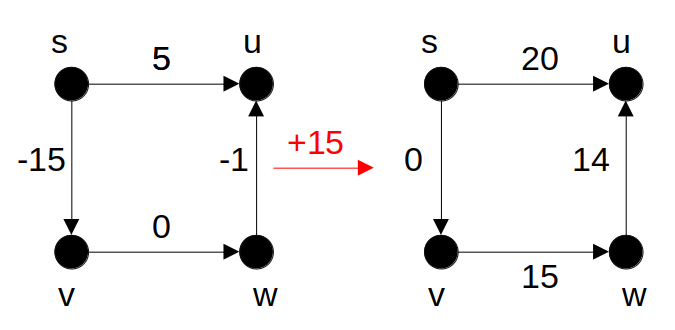
\includegraphics[width=0.4\textwidth]{data/graf_rownowazny_kontrprzyklad.png}
	\caption{  }
	\label{fig:kontrprzyklad_johnson}
\end{figure}

Konstrukcja grafu równoważnego $(G', \omega')$ 
do grafu wejściowego $(G, \omega)$
w algorytmie Johnsona polega na
dodaniu do $G$ wierzchołka $q$, oraz 
dla każdego wierzchołka $v \in V(G)$ krawędzi
skierowanych $qv$ z wagą 0. 

W następnym kroku wywołujemy algorytm Belmmana-Forda
na grafie $(G', w')$ z wierzchołkiem 
startowym $q$ po to, aby utworzyć nową funkcję wagową
na $G$, która zawsze będzie przyjmować wartości 
nieujemne. Umożliwi to zastowanie 
algorytmu Dijsktry. 

\begin{algorithm}[H]
	\caption{Algorytm Johnsona}
	\begin{algorithmic}[1]
		\Procedure{Johnson}{($G, \omega$): graf ważony}
		\State $V' \gets V(G) \cup \{q\}$ 
		\State $E' \gets  E(G) \cup \{qv : v \in V(G)\}$
		\State Skonstruuj graf skierowany $(G', V')$
		\State Zdefiniuj funkcję $w' : E' \to \mathbb{R}$, 
		gdzie 
		\[w'(e) = \begin{cases}
			w(e), &\text{ jeśli } e \in E(G) \\
			0, &\text{ jeśli }  e \not \in E(G)   
		\end{cases}\]
		\State $h \gets \textsc{BellmanFord}((G', w'), q)$
		\State Zdefiniuj funkcję $w'' : E(G) \to \mathbb{R}$, 
		gdzie 
		\[w''(uv) = w(uv) + h(u) - h(v)\]
		\For{$u \in V(G)$}
		\State $d_u = \textsc{Dijsktra}((G, w''), u)$
		\For{$v \in V$}
		\State \textit{odległości}$[u, v] \gets d_u[v] - h[u] + h[v]$
		\EndFor
		\EndFor
		\State \Return \textit{odległości}
		\EndProcedure
	\end{algorithmic}
	\label{Johnson}
\end{algorithm}

Zakładając, że kolejka priorytetowa zastosowana 
w algorytmie Dijsktry jest oparta na kopcach 
Fibonacciego, otrzymujemy złożoność $O(n^2\log n + nm)$. Algorytm 
ten jest szybszy dla grafów rzadkich niż kolejno omawiany 
algorytm Floyda-Warshalla. 

\begin{theorem}[Poprawność algorytmu Johnsona]
	Jeśli $(G, w)$ jest ważonym grafem skierowanym
	bez ujemnych cykli, to algorytm Johnsona dla 
	danych wejściowych $(G, w)$ poprawnie
	rozwiązuje problem najkrótszej ścieżki 
	pomiędzy dowolnymi parami wierzchołków.
	
	\begin{proof}
		Przez $dist_\chi(u, v)$ oznaczmy wagę minimalnej ścieżki
		z wierzchołka $u$ do $v$ przy ważeniu $\chi$ domyślając się, 
		że chodzi o graf $G$ lub $G'$ w zależności od dziedziny $\chi$.
		
		Aby wykazać poprawność aglorytmu Johnsona, 
		musimy udowodnić poniższe obserwacje:
		\begin{enumerate}
			\item Dane wejściowe do 
			algorytmu Bellmana-Forda są poprawne.
			\item Dane wejściowe do 
			algorytmu Dijkstry są poprawne.
			\item Niech $P$ będzie dowolną
			$u$-$v$-ścieżką w grafie $G$ oraz niech $h$
			będzie odwzorowaniem zwróconym przez algorytm
			Belmmana-Forda w linii nr 6. Wtedy
			\[w''(P) = w(P) +  h(u) - h(v).\]
			\item Niech $u, v \in V(G)$, wtedy
			\[dist_{w}(u, v) = dist_{w''}(u, v) - h(u) + h(v).\]
		\end{enumerate}
		
		\paragraph{Dowód obserwacji 1.} Graf ($G$, $w$)
		z założenia nie posiada ujemnych cykli. Ponadto
		dodanie do $G$ wierzchołka $q$ oraz krawędzi skierowanymi
		od $q$ do każdego wierzchołka z $G$ nie może utworzyć
		żadnego nowego cyklu, a więc w szczególności nie może
		w ten sposób powstać żaden ujemny cykl. Oznacza to, że
		$(G', w')$ oraz $q$ to poprawne dane wejściowe
		do algorytmu Bellmana-Forda.
		
		\paragraph{Dowód obserwacji 2.} Niech $uv \in E(G')$. Wtedy prawdą jest, że
		\[dist_{w'}(q, v) \leq dist_{w'}(q, u) + w'(uv),\]
		co w połączeniu z poprawnością algorytmu Belmmana-Forda (tw.
		\ref{bellmanford_proof}) oraz faktem, że 
		$uv \in E(G)$ daje nam
		\[h(v) \leq h(u) + w(uv).\]
		Po przeniesieniu $h(v)$ na prawą stronę otrzymujemy 
		\[0 \leq w(uv) + h(u) - h(v) = w''(uv),\]
		więc każda krawędź grafu ważonego $(G, w'')$ ma
		nieujemną wagę. Wnioskujemy, że wywołanie algorytmu 
		Dijkstry jest poprawne.  
		
		\paragraph{Dowód obserwacji 3.} Niech $P=v_1v_2\dots v_k$, 
		gdzie $v_1 = u$ oraz $v_k = v$ będzie dowolną $u$-$v$-ścieżką
		w grafie $G$. Wtedy 
		\[w''(P) = w''(v_1v_2) + w''(v_2v_3) + \dots + w''(v_{k-1}v_k).\]
		Korzystając z definicji $w''$ otrzymamy
		\[w''(P) = w(v_1v_2) + h(v_1) - (h_2) + 
		w(v_2v_3) + h(v_2) - (h_3) + 
		\dots + w(v_{k-1}v_k) + h(v_{k-1}) - (h_k).\]
		Po uporządkowaniu powyższego dostaniemy
		\[w''(P) = w(P) + w(v_1) - w(v_k) = w(P) + h(u) - h(v),\]
		co należało dowieść.
		
		\paragraph{Dowód obserwacji 4.} Niech $P_{w}$ oraz 
		$P_{w''}$ będą najkrótszymi $u$-$v$-ścieżkami odpowiednio 
		przy ważeniu $w$ oraz $w''$. Korzystając z 
		Obserwacji 3 otrzymujemy
		\[w''(P_{w}) = w(P_{w}) + h(u) - h(v) \leq
		w(P_{w''}) + h(u) - h(v) = w''(P_{w''}),\]
		co wynika, z założenia, że $P_{w}$ to 
		najmniejsza ścieżka w $(G, w)$. 
		
		Z powyższej nierówności oraz z założenia, że $P_{w''}$ to 
		najmniejsza ścieżka w $(G, w'')$ otrzymujemy
		\[w''(P_{w''}) \leq w''(P_{w}) \leq w''(P_{w''}), \]
		\[w''(P_{w''}) = w''(P_{w}).\]
		Po ponownym zastosowaniu obserwacji 3
		\[w''(P_{w''}) = w(P_{w}) + h(u) - h(v),\]
		\[w(P_{w''}) = w''(P_{w''}) - h(u) + h(v).\]
		Dzięki poprawności algorytmu Dijkstry (tw. \ref{dijkstra_proof})
		mamy
		\[dist_{w}(u, v) = dist_{w''}(u, v) - h(u) + h(v).\]
		
		Obserwacje 1, 2 i 4 implikują, że tablica \textit{odległości} zostanie
		wypełniona poprawnie. Jako że algorytm na pewno zakończy pracę,
		dowód poprawności jest kompletny.
	\end{proof} 
\end{theorem}

\subsubsection{Algorytm Floyda-Warshalla}
\begin{algorithm}[H]
	\caption{Algorytm Floyda-Warshalla}
	\begin{algorithmic}[1]
		\Procedure{FloydWarshall}{($G, w$): graf ważony}
		\State Utwórz tablicę odległości o wymiarach $V(G) \times V(G)$
		\For{$i \in V(G)$}
		\For{$j \in V(G)$}
		\If{$ij \in E(G)$}
		\State $\textit{odległości}[i, j] \gets w(ij)$
		\Else
		\State $\textit{odległości}[i, j] \gets \infty$
		\EndIf
		\EndFor
		\EndFor
		\For{$i \in V(G)$}
		\State $\text{odległości}[i, i] \gets 0$
		\EndFor
		\For{$k \in V(G)$}
		\For{$i \in V(G)$}
		\For{$j \in V(G)$}
		\If{$\textit{odległości}[i, j] > \textit{odległości}[i, k] + \textit{odległości}[k, j]$}
		\State $\textit{odległości}[i, j] \gets \textit{odległości}[i, k] + \textit{odległości}[k, j]$
		\EndIf
		\EndFor
		\EndFor
		\EndFor
		\State \Return \textit{odległości}
		\EndProcedure
	\end{algorithmic}
	\label{floydWarshall_alg}
\end{algorithm}

Złożoność powyższego algorytmu to $O(n^3)$.

\begin{theorem}[Poprawność algorytmu Floyda-Warshalla]
	Jeśli $(G, w)$ jest ważonym grafem skierowanym
	bez ujemnych cykli, to algorytm Floyda-Warshalla dla 
	danych wejściowych $(G, w)$ poprawnie
	rozwiązuje problem najkrótszej ścieżki 
	pomiędzy dowolnymi parami wierzchołków.
	
	\begin{proof}
		Oznaczmy przez $d^{(m)}$(i, j) długość najkrótszej
		$i$-$j$-ścieżki, której wewnętrzne wierzchołki 
		należą do zbioru $\{0, 1, 2, \dots, m-1\}$. 
		Ponadto przez
		$\textit{odległości}_{m}[i, j]$ będziemy rozumieli 
		stan tablicy po 
		wykonaniu się $m$-tej iteracji.
		
		\paragraph{Niezmiennik.} Po $l$ iteracjach 
		pętli \textit{for} w linii nr 11, dla każdych wierzchołków
		$i, j \in V(G)$ zachodzi \textit{odległości}$[i,j] \leq d^{(l)}(i,j)$.
		
		\paragraph{Dowód niezmiennika.} Indukcja po liczbie iteracji $l$.
		
		Wartości początkowe spełniają warunek, zatem
		baza indukcyjna jest prawdziwa. 
		
		Przypuśćmy, że $\text{odległości}_{l}[i, j] \leq
		d^{(l)}(i, j)$. Chcemy pokazać, że 
		$\textit{odległości}_{l+1}[i, j] \leq$$ d^{(l+1)}(i, j)$.
		W przypadku, kiedy $d^{(l)}(i,j) =$$ d^{(l+1)}(i,j)$, to
		\[d^{(l+1)}(i,j) = d^{(l)}(i, j) \geq 
		\text{odległości}_l[i, j] \geq \text{odległości}_{l+1}[i, j],\]
		gdzie pierwsza nierówność wynika z założenia indukcyjnego, natomiast
		druga z 14 i 15 linii algorytmu, które implikują, że
		w każdej iteracji wartości w tablicy \textit{odległości} mogą jedynie się zmniejszyć lub
		nie ulec żadnej zmianie.
		
		Rozważmy przypadek kiedy $d^{(l)}(i,j) >$$ d^{(l+1)}(i,j)$. 
		W takiej sytuacji musiała powstać co najmniej jedna 
		$i$-$j$-ścieżka. Każda z nowopowstałych $i$-$j$-ścieżek
		musi zawierać w sobie wierzchołek $l$. Niech 
		$P$ będzie najkrótszą z nich. Zauważmy, że
		\[w(P) = d^{(l+1)}(i, j) = 
		d^{(l+1)}(i, l) + d^{(l+1)}(l, j),\]
		gdzie druga równość wynika z wielokrotnego zastosowania 
		lematu \ref{minpath_subpath}.
		
		Ponadto możemy zauważyć, że $d^{(l+1)}(i, l) = d^{(l)}(i, l)$ 
		oraz $d^{(l+1)}(l, j) = d^{(l)}(l, j)$. Wynika to z faktu, że
		najkrótsza ścieżka zaczynająca się w $l$, której wnętrze składa się z wierzchołków 
		$\{0, 1, 2, \dots, l-1\}$,
		nie może być gorsza niż najkrótsza ścieżka, której 
		wnętrze składa się z wierzchołków 
		$\{0, 1, 2, \dots, l-1, l\}$.
		
		Zatem ostatecznie:
		\begin{gather*}
		\text{odległości}_{l+1}[i,j] \leq 
		\text{odległości}_{l}[i,l] + \text{odległości}_{l}[l,j] \leq
		\\
		\leq d^{(l)}(i, l) + d^{(l)}(l, j) = d^{(l+1)}(i, l) + d^{(l+1)}(l, j) = d^{(l+1)}(i, j),
		\end{gather*}
		gdzie pierwsza nierówność wynika z 14 oraz 15 linii algorytmu,
		natomiast druga -- z założenia indukcyjnego.
		
		Na mocy indukcji matematycznej niezmiennik jest prawdziwy.
		
		\paragraph{Stwierdzenie. } W każdym momencie działania algorytmu
		dla każdego wierzchołka $v \in V(G)$ zachodzi 
		\[\textit{odległość}[v] \geq d(v).\]
		
		\paragraph{Dowód stwierdzenia.} Indukcja po liczbie iteracji $l$.
		
		Dla zerowej liczby wywołań teza jest spełniona, a 
		zatem baza indukcyjna jest prawdziwa.
		
		Przyjmijmy, że jeśli $\textit{odległości}_l[i, j] \geq d(i, j)$
		jest prawdą, to $\textit{odległości}_{l+1}[i, j] \geq d(i, j)$
		również musi być prawdziwe.
		
		Jeśli $\textit{odległość}_{l+1}[i, j] = \textit{odległość}_{l}[i, j]$,
		to korzystając z założenia indukcyjnego, możemy zakończyć dowód.
		
		Rozważmy przypadek, kiedy 
		$\textit{odległość}_{l+1}[i, j] < \textit{odległość}_{l}[i, j]$. 
		Aby ten przypadek zaszedł, musiały wykonać się linijki 14 i 15.
		Oznacza to, że 
		\[\textit{odległość}_{l+1}[i, j] = \textit{odległość}_{l}[i, l+1] 
		+ \textit{odległość}_{l}[l+1, j] \geq d(i, l+1) + d(l+1, j)
		\geq d(i, j),\]
		gdzie pierwsza nierówność wynika z założenia indukcyjnego,
		natomiast druga z faktu, że $d(i, j)$ oznacza
		długość najkrótszej ścieżki.
		
		Na mocy indukcji matematycznej stwierdzenie jest prawdziwe.
		
		Stwierdzenie oraz niezmiennik implikują, że 
		dla każdej pary wierzchołków
		$i, j \in V(G)$ prawdą jest, że 
		\[\textit{odległość}_n[i,j] \leq d^{(n)}(i, j) = d(i, j) \leq \textit{odległość}_n[i,j],\]
		a zatem
		\[\textit{odległość}_n[i,j] = d(i, j),\]
		co kończy dowód. \qedhere
	\end{proof} 
	\label{floydWarshall_proof}
\end{theorem}

\subsubsection{Podsumowanie}